\chapter{Objetivos y metodología de desarrollo}

En este capítulo se define el objetivo principal del proyecto, junto con los objetivos específicos que permitirán alcanzarlo de manera efectiva.

Asimismo, se detallará la metodología de trabajo utilizada en el desarrollo de la plataforma, describiendo los enfoques y herramientas empleados en el desarrollo para este trabajo.
\newpage
\section{Objetivos}

Para alcanzar una meta, es fundamental definir con precisión qué se desea lograr y establecer los pasos y condiciones necesarios para lograrlo de manera efectiva.

El \textbf{objetivo principal} de este trabajo es \textbf{desarrollar un sistema de recomendación de videojuegos} que ofrezca sugerencias personalizadas y alineadas con las preferencias y necesidades del usuario.

Para alcanzar este objetivo de manera óptima, es esencial cumplir con los siguientes objetivos secundarios:

\begin{itemize}
    \item \textbf{Diseñar una interfaz clara, intuitiva y accesible} para garantizar una experiencia de usuario fluida y sin barreras.
    \item \textbf{Mejorar la personalización del sistema} mediante el aprendizaje y almacenamiento de las interacciones del usuario, así como la integración de datos provenientes de otras plataformas.
    \item \textbf{Implementar y coordinar múltiples modelos de lenguaje} para optimizar la precisión y diversidad de las recomendaciones.
    \item \textbf{Incorporar factores adicionales en las recomendaciones}, como disponibilidad del juego, requisitos técnicos, accesibilidad y presupuesto del usuario.
    \item \textbf{Facilitar la actualización del sistema} con nuevas tendencias y lanzamientos en el sector de los videojuegos, considerando las limitaciones en el entrenamiento de los modelos de lenguaje.
    \item \textbf{Optimizar el rendimiento del sistema} para ofrecer respuestas rápidas, precisas y justificadas, mejorando la experiencia de usuario.
    \item \textbf{Garantizar la privacidad y seguridad de los datos} mediante buenas prácticas de almacenamiento y procesamiento de información.
\end{itemize}

El cumplimiento de estos objetivos asegurará el desarrollo de un sistema de recomendación eficaz y adaptado a las necesidades del usuario.
\newpage
\section{Metodología de desarrollo}

Para el \textbf{desarrollo} de la plataforma, se ha adoptado un enfoque basado en \textbf{metodologías ágiles}, priorizando la \textbf{flexibilidad} y la \textbf{adaptación} continua a los desafíos y necesidades emergentes a lo largo del proceso. Las metodologías ágiles se centran en la entrega \textbf{incremental} de valor, permitiendo \textbf{ajustes rápidos y frecuentes} en función de los comentarios, necesidades e inconvenientes surgidos a lo largo del desarrollo. Este enfoque se caracteriza por ciclos de trabajo cortos, denominados "\textbf{sprints}", en los cuales se planifica, ejecuta, prueba y evalúa el progreso de manera continua, asegurando la flexibilidad y la rápida implementación de cambios.

La \textbf{planificación} inicial fue un proceso caótico. Aunque comencé con una idea general del proyecto, a medida que avanzaba, fui desarrollando cada sección de la memoria de forma paralela, sin perder de vista cómo se conectaban entre sí los capítulos y cómo se iban integrando los distintos elementos del trabajo. La planificación fue en constante evolución, adaptándose a los tiempos limitados y a los factores externos imprevistos, lo que permitió cumplir con los objetivos, aunque de manera más flexible y con ajustes frecuentes en el camino.

A medida que el desarrollo fue avanzando, la planificación se fue optimizando mediante el establecimiento de objetivos más concretos y plazos más definidos para cada sprint. De esta manera, se lograron entregas parciales de la plataforma, que permitieron validar la funcionalidad y realizar mejoras progresivas en cada ciclo. Además, la iteración continua y la retroalimentación temprana de las soluciones implementadas ayudaron a reducir riesgos y garantizar la calidad del producto final.

La planificación se podría resumir en este diagrama de Gantt:

\begin{figure}[H]
	\centering
	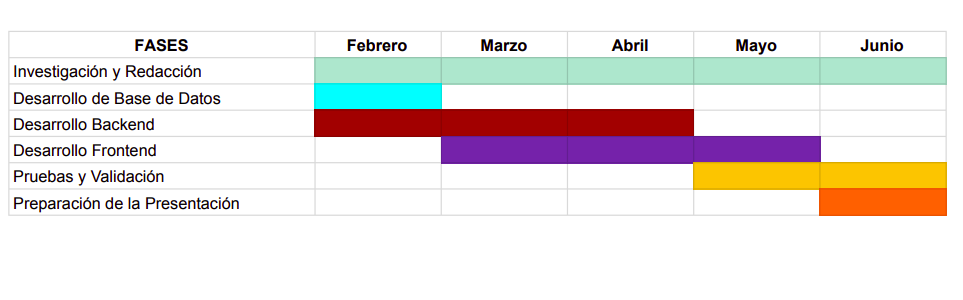
\includegraphics[width=1\linewidth]{imagenes/diagrama.png}
	\caption[\textbf{Planificación en diagrama de Gantt}.]{\textbf{Planificación en diagrama de Gantt}. Apreciamos como el proyecto se ha realizado a través de los meses. La memoria y la investigación son apartados que evolucionan continuamente. Los distintos elementos de la aplicación se desarrollan por partes, pero en ciertos puntos se integran de forma paralela. Las pruebas y presentación se realiza al final, pero durante todo el proceso se tiene en mente.}
	\label{diagrama}
\end{figure}

Sin embargo, es importante volver a señalar que, debido a mis circunstancias personales, no pude dedicarle mucho tiempo a la organización temporal del proyecto. En mi caso, la gestión del tiempo no ha sido un aspecto en el que pudiera destacar, ni en este trabajo ni en otros aspectos de toda mi vida. Por lo tanto, preferí concentrarme en lo verdaderamente importante: la realización efectiva del trabajo, sin gastar tiempo innecesario en crear planificaciones detalladas solo para cumplir con una formalidad. La prioridad fue avanzar en el desarrollo y en los resultados concretos, adaptándome a lo que surgiera en el camino. \textit{\textbf{Carpe Diem}}.


La \textbf{investigación} ha sido fundamental en la metodología de trabajo, recurriendo a documentación oficial, artículos técnicos y foros especializados para resolver dudas y optimizar la implementación. Además, se adoptó un enfoque práctico basado en la experimentación, probando diversas soluciones y herramientas para garantizar el correcto funcionamiento de la plataforma y su integración.

El uso de herramientas como \textit{ChatGPT} facilitó la corrección ortográfica, la mejora de la redacción y la traducción de textos en otros idiomas, acelerando así el proceso de adquisición de conocimiento y optimizando el tiempo dedicado a la investigación.

\subsection{Presupuesto}

Dado que el proyecto se ha desarrollado de manera autónoma y sin recursos financieros dedicados, los \textbf{costes} asociados se limitan al tiempo invertido, el uso de mis recursos propios, como ordenador y wifi, y al uso de herramientas gratuitas. A continuación, se detalla el presupuesto estimado basado en los costes de un desarrollador informático y los recursos utilizados que podría adecuarse a una empresa:

\begin{itemize}
    \item \textbf{Coste del desarrollador informático:} Según los estándares actuales, el coste medio por hora de un informático en España para un trabajo de este tipo es de aproximadamente 15,27€ por hora\cite{sueldo}. Dado que un TFG dura 300 horas, el cálculo sería el siguiente:
    \[
    300 \, \text{horas} \times 15,27 \, \text{€} = 4.581 \, \text{€}
    \]
    Este coste es aproximado y puede variar dependiendo de la experiencia y la localización del profesional.

    \item \textbf{Equipo informático:} El coste estimado de un ordenador adecuado para el desarrollo de software es de aproximadamente 1.420€, más un ratón de unos 26 €, considerando un equipo de gama media-alta, como es mi caso. Aunque como este desarrollo no requiere de una GPU de altas prestaciones, ya que no se genera casi gráficos ni se hacen muchos cálculos, es perfectamente viable usar un equipo más barato que no tenga una GPU dedicada, o que esta sea una básica destinada a la ofimática.

    \item \textbf{Consumo de electricidad:} El consumo de un ordenador durante un periodo de 300 horas puede suponer un coste de aproximadamente 42€ (suponiendo un consumo medio de 0.2 kWh (portátil enchufado más una lámpara) por hora\cite{luz} y un coste de unos 0.14€ por kWh). El coste de la electricidad es un factor muy importante a tener en cuenta. Aunque se ha estimado un gasto general, es necesario señalar que este coste puede ser en realidad mayor debido a las tarifas diferenciadas por franjas horarias, las cuales, lamentablemente, están bastante elevadas en las franjas activas. Esta situación resulta aún más agravante al considerar el aumento constante de los precios de la energía, lo que incrementa considerablemente los costes operativos de los proyectos que requieren un uso constante de equipos eléctricos. Es incluso más vergonzoso ver cómo la precariedad de nuestros dirigentes —más interesados en montar un circo entre ellos, que en hacer las cosas bien y con responsabilidad— nos deja sin luz casi un día entero, costándonos a muchos una valiosa jornada de trabajo, e incluso, en algunos casos, algo aún peor: la vida. Es lamentable comprobar cómo no hay consecuencias para los culpables, sino aplausos de sus fieles, sumisos como ganado.


    \item \textbf{Conexión a internet:} El coste de un servicio básico de internet(sin contar las líneas móviles) es de alrededor de 30 € con MasMovil. Suponiendo que el proyecto dure 6 meses, el coste estimado de la conexión a internet sería:
    \[
    30 \, \text{€} \times 6 \, \text{meses} = 180 \, \text{€}
    \]

    \item \textbf{Herramientas y servicios en línea:} Las herramientas empleadas, como \textit{GitHub}, \textit{LangChain}, \textit{LangGraph} y \textit{ChatGPT}, fueron utilizadas en sus versiones gratuitas, lo que ha permitido minimizar los costes. No obstante, en un entorno profesional, estos servicios pueden tener un coste mensual que suele variar entre 10€ y 100€ dependiendo de las funcionalidades requeridas.

    \item \textbf{Juego en Steam:} Steam requiere un gasto directo de al menos 5 dólares para habilitar ciertas funciones, como la lista de amigos, actividades o el acceso a sus APIs. En mi caso, no había alcanzado ese umbral, ya que suelo adquirir juegos mediante plataformas de keys, que generalmente ofrecen mejores precios y no dependen de los periodos de rebajas oficiales de Steam. Compré Cult of the Lamb por 11,49€, lo que activó esas funcionalidades.
    
\end{itemize}

\textbf{Resumen del presupuesto estimado:}

\begin{itemize}
    \item \textbf{Coste del desarrollador informático:} 4.581€
    \item \textbf{Equipo informático:} 1.446€ (incluyendo ratón)
    \item \textbf{Consumo de electricidad:} 42€
    \item \textbf{Conexión a internet:} 180€
    \item \textbf{Herramientas en línea (versión gratuita):} 0€
    \item \textbf{Juego de Steam:} 11.49€
\end{itemize}

\textbf{Total estimado de costes (sin incluir costes de servicios pagos):} 6.260.49€

Este presupuesto refleja el coste real de desarrollar el proyecto de manera autónoma, sin considerar gastos adicionales relacionados con licencias de software, servicios profesionales o materiales externos.

\textbf{Conclusión}


La metodología ágil permitió una planificación flexible y adaptable a los retos del proyecto, lo que garantizó el éxito del desarrollo de la plataforma. Además, el uso de herramientas gratuitas y la optimización de recursos han permitido mantener los costes del proyecto en niveles razonables, asegurando que el objetivo final se alcanzara dentro de los plazos establecidos, sin comprometer la calidad del trabajo realizado.


